We evaluate three questions: whether restricted adaptation improves object prediction and closed-loop planning across adaptation-data budgets under diagnosed joint locks; whether selective readout and independent recurrence retain object corrections while preserving the reference robot forecast; and whether the controller completes pushes under physical joint locks.




\subsection{Simulation benchmark and quantitative comparison}
\noindent\hspace*{1em}\textbf{Task setup.} We evaluate planar box pushing under five single-joint locks in MuJoCo~\cite{todorov2012mujoco}. The object has a fixed orientation. Dynamics settings comprise nominal conditions, doubled damping, 70\% actuator gain, and the combination of the latter two. Each trajectory starts from an independent reset with checks on support geometry and joint limits. Training, validation, and test sets contain 50,000, 2,000, and 6,000 trajectories, respectively.

\noindent\hspace*{1em}\textbf{Implementation and training.} The robot encoder uses a five-node chain graph~\cite{battaglia2016interaction,sanchezgonzalez2020learning}, hidden width 136, two message-passing rounds and 136-unit GRUs~\cite{cho2014gru}. SiLU~\cite{elfwing2018silu} networks have widths $6\to136\to136$ (encoder), $272\to136\to136$ (messages), $136\to136\to2$ (joint head), and $140\to136\to4$ (object head). The residual uses a 12-dimensional descriptor and a 16-unit Tanh hidden layer. Its inputs are previous/next pusher positions, their difference, next-pusher-to-object displacement, object velocity, and pre/post-transition contact gates. Capsule radii are 12 and 8 mm; the object box is 40 mm; $\tau=-0.005$ m and $\epsilon=0.002$ m. The state dimension is $d_s=14$. Normalization scales are 0.1 rad, 1 rad/s, 0.03 m, and 0.1 m/s for joint position/velocity and object position/velocity. Training uses $E=10$ epochs, with $H_e=10$ for the first five and $H_e=25$ thereafter; each trajectory supplies one random contiguous window per epoch. Validation uses $H_v=25$, including the initial checkpoint.

\noindent\hspace*{1em}\textbf{Baselines.} We compare three adaptation variants of the same pretrained model to evaluate the effect of adaptation scope. Carrier adapts the object head with robot parameters fixed; LockPusher adds a geometric object residual while retaining the reference robot forecast; Global permits residual corrections to all state coordinates. The methods share pretrained weights, data, optimization budgets, and adaptation seeds 7, 17, and 27. Checkpoints are selected by 25-step validation object-position error. This comparison tests the contribution of the object residual and the effect of also adapting robot coordinates.

\noindent\hspace*{1em}\textbf{Evaluation protocol.} All methods solve the same 1,200 initial-state--goal problems, with a mean initial goal distance of 65 mm. Each planning cycle selects among 128 candidates, executes ten steps, and obtains a new observation. Five cycles give 0.25 s of execution. We report per-coordinate object-position RMSE at step 50, mean final goal distance, and the fraction of trials with a final goal distance of less than 1 mm. The matched full-data comparison is summarized in Table~\ref{tab:core-results}.

\begin{table}[!tbp]\centering\small

\setlength{\tabcolsep}{4pt}
\begin{tabular}{lrrr}\toprule
Method & \shortstack{Object RMSE\\(mm)} & \shortstack{Goal distance\\(mm)} & \shortstack{Success\\(\%)}\\\midrule
Carrier &5.07&3.32&47.84\\
Global &2.98&2.06&65.29\\
LockPusher &\textbf{1.58}&\textbf{1.43}&\textbf{76.53}\\\bottomrule
\end{tabular}\caption{Full-data simulation results averaged over three training seeds. LockPusher achieves lower prediction and goal errors and higher task success than both baselines. RMSE denotes root mean squared error.}
\label{tab:core-results}
\end{table}
\noindent\hspace*{1em}\textbf{Results.} LockPusher achieves 1.58 mm object-position RMSE, 1.43 mm final goal distance, and 76.53\% success. Relative to Global, prediction error decreases by 46.98\% and success increases by 11.24 percentage points. Thus, restricting robot-side adaptation can accompany improved object prediction and closed-loop task performance in this benchmark.



\noindent\hspace*{1em}\textbf{Effect of adaptation-data budget.} We evaluate ten adaptation-data fractions from 10\% to 100\% and retain the same evaluation tasks at each fraction. Figure~\ref{fig:adaptation-data}(a,c,e) reports the mean and one standard deviation over three training seeds. LockPusher achieves lower mean object-position RMSE and final goal distance, together with higher mean task success, at every evaluated fraction. Its simulation advantage therefore extends across the tested adaptation budgets.

\begin{figure}[!tb]
\centering
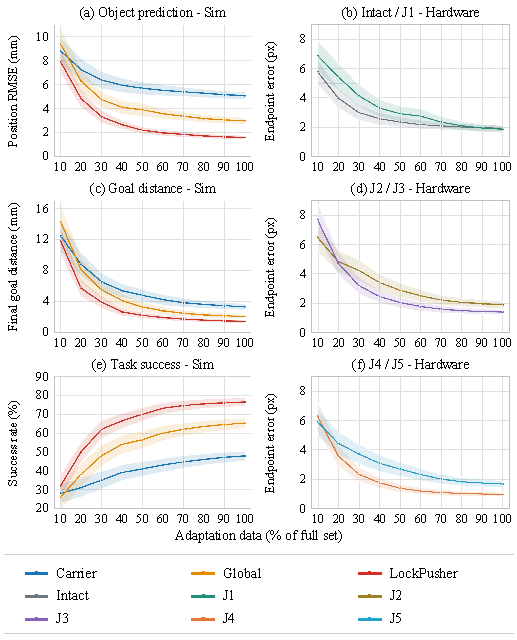
\includegraphics[width=\columnwidth]{figures/submission-layout-20260915-191848/adaptation_data_single_column.pdf}
\caption{LockPusher improves simulation prediction and task performance across the tested data budgets (left); hardware endpoint error decreases as adaptation data increase (right). Shading shows mean $\pm1$ SD over three training seeds. Hardware 100\% denotes 100 adaptation trajectories per condition.}
\label{fig:adaptation-data}
\end{figure}

\begin{figure*}[!t]
\centering
\includegraphics[width=\textwidth]{figures/lockpusher_revision/all18_oblique.pdf}
\caption{LockPusher performs nonprehensile pushing with the intact arm and under five single-joint locks. Three recorded executions per condition illustrate its ability to continue object manipulation with different joints immobilized.}
\label{fig:hardware-oblique}
\end{figure*}

\subsection{Module analysis and ablations}
\noindent\hspace*{1em}\textbf{Object adaptation and reference preservation.} We test whether selective readout and independent recurrence retain object corrections while controlling their effect on robot predictions. With fixed checkpoints and paired inputs, the two experiments change the returned coordinates and the rollout feedback, respectively.

\noindent\hspace*{1em}\textbf{Effect of selective readout.} Using the same historical checkpoints, we compare full-state intervention and selective readout. Both readouts use the same object prediction, so both retain the 16.74\% mean reduction in composite object-state RMSE; they differ in the robot coordinates returned to the planner. Full-state intervention reduces free-state error in 24 combinations and increases it in three, by up to 6.20\%. Selective readout retains Carrier's free-state and pusher errors in all 27 combinations (Table~\ref{tab:historical-publication}).

\begin{table}[!tbp]\centering\small

\setlength{\tabcolsep}{3pt}
\begin{tabular}{lrrrr}\toprule
& \shortstack{Object RMSE\\reduction (\%)} & \shortstack{Free\\worse} & \shortstack{Max. free\\increase (\%)} & \shortstack{Free/FK\\match}\\\midrule
Carrier & 0.00 & 0/27 & 0.00 & 27/27\\
Full-state & 16.74 & 3/27 & 6.20 & 0/27\\
Selective & 16.74 & 0/27 & 0.00 & 27/27\\
\bottomrule\end{tabular}\caption{Historical selective-readout ablation across 27 combinations. Both readouts retain the same object-error reduction, while selective readout preserves the reference robot prediction in every combination. Free worse counts increased free-state errors; Free/FK match counts unchanged free-state and forward-kinematics pusher errors. Changes are relative to Carrier.}
\label{tab:historical-publication}
\end{table}
\noindent\hspace*{1em}\textbf{Effect of independent recurrence.} We fix weights and inputs and compare shared-state feedback with independent recurrence on 12 trajectories in each of seven conditions, totaling 84 trajectories. Three checkpoints, seven conditions, and horizons of 10, 25, and 50 steps give 63 evaluation combinations. Independent recurrence preserves the reference robot prediction in all 63 combinations, whereas shared feedback changes it in all 63; object-position and velocity RMSE are identical. Robot error decreases in 60 combinations and increases in three. The historical reset protocol awaits independent physical-validity checks.




\subsection{Real-world experiments}
\noindent\hspace*{1em}\textbf{Hardware setup.} The hardware platform and recorded intact-arm and joint-lock executions are shown in Figs.~\ref{fig:real-scene} and~\ref{fig:hardware-oblique}; for the deployed controller, we execute three pushes on the intact arm and under each of the J1--J5 locks, for 18 trials. Each target displacement is 40 image pixels, approximately 51.2 mm under the calibration used for this batch. The controller uses the seed-27 deployment weights and evaluates at least 10,000 joint-reference sequences over 50 steps. It executes the selected reference with a 5-degree/s speed limit and replans from a new observation. Repetitions within each condition reuse a preparation candidate set.
\begin{figure}[!t]\centering
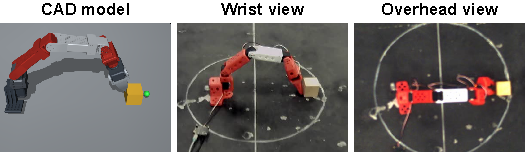
\includegraphics[width=\columnwidth]{figures/hardware-aligned-20260915-200334/environment_plate.pdf}
\caption{We impose joint locks on the same physical arm and record nonprehensile pushing with wrist and overhead cameras.}\label{fig:real-scene}
\end{figure}


\noindent\hspace*{1em}\textbf{Evaluation.} Figure~\ref{fig:hardware-sequence} illustrates the image-space criterion. A trial succeeds when target error is at most two pixels on each image axis in three distinct, consecutive reliable frames. Object endpoint error is computed separately as the norm of the coordinate-wise median XY error over the final ten frames. Table~\ref{tab:hardware-scores} reports both object endpoint error and task outcomes.
\begin{figure}[!t]\centering
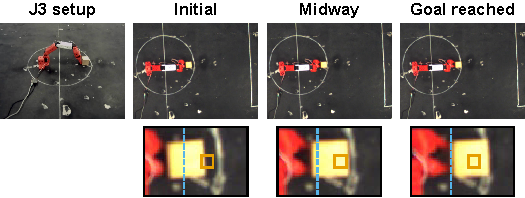
\includegraphics[width=\columnwidth]{figures/hardware-aligned-20260915-200334/hardware_sequence.pdf}
\caption{Under a J3 joint lock, our controller uses visual replanning to push the object toward its goal and confirms arrival through the center-point error in three consecutive frames.}\label{fig:hardware-sequence}
\end{figure}


\begin{table}[!tbp]\centering\small

\begin{tabular}{lrr}\toprule
Condition & \shortstack{Object endpoint error\\mean (px)} & Successes/trials\\\midrule
Intact &1.94&3/3\\
J1 &1.88&3/3\\
J2 &1.92&3/3\\
J3 &1.43&3/3\\
J4 &0.97&3/3\\
J5 &1.68&3/3\\
\midrule All &1.64&18/18\\\bottomrule
\end{tabular}\caption{Real-world results for 40-pixel target displacements. Each success entry gives successful trials out of three attempts. LockPusher completes all tested pushes across the intact arm and five joint-lock conditions; endpoint errors are condition means in pixels.}
\label{tab:hardware-scores}
\end{table}


\noindent\hspace*{1em}\textbf{Pushing under joint locks.} The intact arm and all five single-joint-lock conditions complete three pushes each, giving 18 successful trials. Mean object endpoint error is approximately 1.64 pixels, with condition means from 0.97 to 1.94 pixels. 

The same data-budget study continues on hardware: we collect 100 complete adaptation trajectories for each of the intact-arm and five joint-lock conditions, totaling 600 trajectories. Each fraction uses 10--100 trajectories from its own condition and is evaluated on the same test tasks. Figure~\ref{fig:adaptation-data}(b,d,f) reports means and one standard deviation over three training seeds. Mean object endpoint error decreases as adaptation data increase in all six conditions, extending the simulation trend to physical execution. 


